\documentclass{standalone}
\usepackage{tikz}
\usepackage{ifthen}
\usepackage{hsbcommon}
\begin{document}
    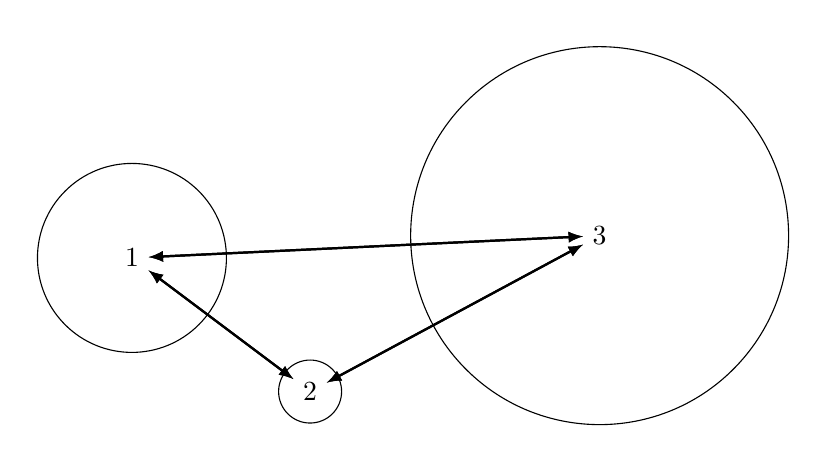
\begin{tikzpicture}[scale=0.4,rotate=-45]
        \foreach[count=\i] \x/\y/\Z in
            {0/1/3,
            7/2/1,
            10/12/6%
            }{
            \node (\i) at  (\x,\y) {\i};
            \draw (\x,\y) circle (\Z);
            }
        \foreach \i in {1,2,3}
            \foreach \ii in {1,2,3}
                \ifthenelse{\equal{\i}{\ii}}{}
                {
                \draw[thick, <->, >=latex]  
                 (\i) -- 
                (\ii);                
                };
    
    \end{tikzpicture}
\end{document}

    % \begin{equation}
    %     T_y=A\times Y_i \times \frac{Y_j}{D_{ij}}
    % \end{equation}

    % \begin{description}
    %     \item[A] const.
    %     \item[Y] GDP (of $i$ or $j$ )
    %     \item[D] Distance (between $i$ and $j$)
    % \end{description}